\documentclass[11pt,twocolumn]{article}

% ============================================================
% Page layout
% ============================================================
\usepackage[letterpaper,margin=0.75in]{geometry}
\usepackage{microtype}
\usepackage{parskip}
\setlength{\columnsep}{0.25in}

% ============================================================
% Core math packages
% ============================================================
\usepackage{amsmath}
\usepackage{mathtools}

% ============================================================
% Fonts: compile with LuaLaTeX
% ============================================================
\usepackage{fontspec}
\usepackage{unicode-math}

\setmainfont{DejaVu Serif}
\setsansfont{DejaVu Sans}
\setmonofont{DejaVu Sans Mono}
\setmathfont{Latin Modern Math}

% Do NOT load amssymb, amsfonts, or bm with unicode-math.
% unicode-math already defines many AMS-style symbols.
% Use \symbfit, \symbf, and \symbfsf instead of \bm.

% ============================================================
% Extra math utilities
% ============================================================
\usepackage{tensor}
\usepackage{cancel}

% ============================================================
% Tables
% ============================================================
\usepackage{booktabs}
\usepackage{array}
\usepackage{tabularx}
\usepackage{multirow}
\usepackage{siunitx}

\sisetup{
  detect-all,
  per-mode=symbol,
  exponent-product=\cdot
}

% ============================================================
% Figures, SVG, PGF/TikZ plots
% ============================================================
\usepackage{graphicx}
\usepackage{svg}
\usepackage{tikz}
\usepackage{pgfplots}
\usepackage{stfloats}

\pgfplotsset{compat=1.18}

\usetikzlibrary{
  arrows.meta,
  calc,
  positioning,
  matrix,
  decorations.pathmorphing
}

% ============================================================
% Captions and references
% ============================================================
\usepackage{caption}
\usepackage{subcaption}
\usepackage[hidelinks]{hyperref}
\usepackage[nameinlink,noabbrev]{cleveref}

% ============================================================
% Common math macros
% ============================================================

% Number systems and spaces
\newcommand{\N}{\mathbb{N}}
\newcommand{\Z}{\mathbb{Z}}
\newcommand{\Q}{\mathbb{Q}}
\newcommand{\R}{\mathbb{R}}
\newcommand{\C}{\mathbb{C}}

\newcommand{\Ltwo}{L^2}
\newcommand{\Lp}[1]{L^{#1}}
\newcommand{\Hsob}[1]{H^{#1}}
\newcommand{\Cinfty}{C^\infty}

% Scalars, vectors, matrices, tensors
% unicode-math-native bold notation; works for Greek too.
\newcommand{\scal}[1]{#1}
\newcommand{\vct}[1]{\symbfit{#1}}   % bold italic vector
\newcommand{\mat}[1]{\symbf{#1}}     % bold upright matrix
\newcommand{\ten}[1]{\symbfsf{#1}}   % bold sans-serif tensor

% Unit vectors
\newcommand{\ihat}{\hat{\vct{i}}}
\newcommand{\jhat}{\hat{\vct{j}}}
\newcommand{\khat}{\hat{\vct{k}}}

% Matrix operations
\newcommand{\T}{^{\mathsf{T}}}
\newcommand{\inv}{^{-1}}
\newcommand{\tr}{\operatorname{tr}}
\newcommand{\diag}{\operatorname{diag}}
\newcommand{\rank}{\operatorname{rank}}
\newcommand{\nullspace}{\operatorname{null}}
\newcommand{\range}{\operatorname{range}}
\newcommand{\determinant}{\operatorname{det}}

% Norms and inner products
\newcommand{\norm}[1]{\left\lVert #1 \right\rVert}
\newcommand{\abs}[1]{\left\lvert #1 \right\rvert}
\newcommand{\inner}[2]{\left\langle #1, #2 \right\rangle}

% Differentials and derivatives
\newcommand{\dd}{\,\mathrm{d}}
\newcommand{\pd}{\partial}

\newcommand{\dv}[2]{\frac{\mathrm{d} #1}{\mathrm{d} #2}}
\newcommand{\dvtwo}[2]{\frac{\mathrm{d}^2 #1}{\mathrm{d} #2^2}}
\newcommand{\pdv}[2]{\frac{\partial #1}{\partial #2}}
\newcommand{\pdvtwo}[2]{\frac{\partial^2 #1}{\partial #2^2}}

% Vector calculus
\newcommand{\grad}{\nabla}
\newcommand{\divg}{\nabla \cdot}
\newcommand{\curlop}{\nabla \times}
\newcommand{\rot}{\nabla \times}
\newcommand{\laplace}{\Delta}

% Matrix exponential
\newcommand{\expm}{\operatorname{expm}}

% Complex numbers
\newcommand{\ii}{\mathrm{i}}
\newcommand{\Real}{\operatorname{Re}}
\newcommand{\Imag}{\operatorname{Im}}

% Fourier and Laplace transforms
\newcommand{\FT}{\mathcal{F}}
\newcommand{\IFT}{\mathcal{F}^{-1}}
\newcommand{\LT}{\mathcal{L}}
\newcommand{\ILT}{\mathcal{L}^{-1}}
\newcommand{\fourier}[1]{\widehat{#1}}

% Probability and statistics
\newcommand{\E}{\mathbb{E}}
\newcommand{\Var}{\operatorname{Var}}
\newcommand{\Cov}{\operatorname{Cov}}
\newcommand{\Prob}{\mathbb{P}}
\newcommand{\Normal}{\mathcal{N}}

% Quaternions
\newcommand{\quat}[1]{\mathbf{#1}}
\newcommand{\qconj}[1]{#1^{*}}
\newcommand{\qinv}[1]{#1^{-1}}
\newcommand{\qmul}{\otimes}

% Stochastic calculus
\newcommand{\Wiener}{W_t}
\newcommand{\ito}{\mathrm{d}}

% Numerical methods
\newcommand{\bigO}{\mathcal{O}}

% Logic notation
% Avoid generic names like \And, \Or, \Not because they collide with packages/classes.
\newcommand{\lforall}{\forall}
\newcommand{\lexists}{\exists}
\newcommand{\lexistsone}{\exists!}
\newcommand{\lnexists}{\nexists}

\newcommand{\limplies}{\Rightarrow}
\newcommand{\limpliedby}{\Leftarrow}
\newcommand{\liff}{\Leftrightarrow}

\newcommand{\landop}{\mathbin{\land}}
\newcommand{\lorop}{\mathbin{\lor}}
\newcommand{\lnotop}{\neg}

\newcommand{\ltherefore}{\therefore}
\newcommand{\lbecause}{\because}

% Avoid unicode-math / mathtools \coloneqq warning.
\newcommand{\definedas}{\mathrel{:=}}
\newcommand{\definedasalt}{\mathrel{\triangleq}}

% ============================================================
% Metadata
% ============================================================
\title{A Survival Guide to Modern Mathematical Notation}
\author{Mikhail Grushinskiy}
\date{\today}

\begin{document}

\maketitle

\begin{abstract}
This short guide introduces the notation commonly used in modern mathematics,
physics, engineering, control theory, signal processing, and numerical modeling.
It is not a complete mathematics textbook. Its purpose is to make symbols
readable: sets, logic, vectors, matrices, tensors, functions, operators,
calculus, probability, Fourier transforms, quaternions, differential equations,
and numerical methods.
\end{abstract}

\section{Mathematics as a Symbolic Language}

Mathematical notation is a compressed language for describing structure.
A single expression can describe numbers, geometry, dynamics, uncertainty,
or an entire system of equations.

For example,
\[
\mat{A}\vct{x}=\vct{b}
\]
says that a matrix \(\mat{A}\) acts on a vector \(\vct{x}\) to produce another
vector \(\vct{b}\).

Different visual styles usually signal different kinds of objects:
\[
x,
\qquad
\vct{x},
\qquad
\mat{A},
\qquad
\ten{T},
\qquad
f,
\qquad
\mathcal{L}.
\]

In this document, the convention is:
\[
\text{scalar } x,
\qquad
\text{vector } \vct{x},
\qquad
\text{matrix } \mat{A},
\qquad
\text{tensor } \ten{T},
\qquad
\text{operator } \mathcal{L}.
\]

\section{Numbers, Sets, and Spaces}

The most common number systems are
\[
\N \subset \Z \subset \Q \subset \R \subset \C.
\]

Here,
\(\N\) denotes natural numbers,
\(\Z\) integers,
\(\Q\) rational numbers,
\(\R\) real numbers,
and \(\C\) complex numbers.

A real scalar is written
\[
x \in \R.
\]

A real vector of length \(n\) is written
\[
\vct{x} \in \R^n.
\]

A real matrix with \(m\) rows and \(n\) columns is written
\[
\mat{A} \in \R^{m \times n}.
\]

A domain is often denoted by \(\Omega\):
\[
\Omega \subset \R^n.
\]

Its boundary is written
\[
\partial \Omega.
\]

\section{Logic and Quantifiers}

Modern mathematics uses logical symbols to state assumptions, definitions,
theorems, and proofs compactly.

\subsection{Universal and Existential Quantifiers}

The symbol \(\forall\) means ``for all'':
\[
\forall x \in X,\quad P(x).
\]

This means that the statement \(P(x)\) is true for every element \(x\)
in the set \(X\).

The symbol \(\exists\) means ``there exists'':
\[
\exists x \in X
\quad
\text{such that}
\quad
P(x).
\]

This means that at least one element \(x\) in \(X\) satisfies \(P(x)\).

The symbol \(\exists!\) means ``there exists exactly one'':
\[
\exists! x \in X
\quad
\text{such that}
\quad
P(x).
\]

For example,
\[
\exists! x \in \R
\quad
\text{such that}
\quad
x+3=0.
\]

The symbol \(\nexists\) means ``there does not exist'':
\[
\nexists x \in \R
\quad
\text{such that}
\quad
x^2+1=0.
\]

This statement is true over \(\R\), but not over \(\C\).

\subsection{Implication and Equivalence}

Implication is written
\[
P \Rightarrow Q.
\]

This means: if \(P\) is true, then \(Q\) is true.

The reverse implication is written
\[
Q \Rightarrow P.
\]

Logical equivalence, or ``if and only if'', is written
\[
P \Leftrightarrow Q.
\]

This means that both directions hold:
\[
P \Rightarrow Q
\qquad
\text{and}
\qquad
Q \Rightarrow P.
\]

For example,
\[
\mat{A} \text{ is invertible}
\Leftrightarrow
\determinant(\mat{A}) \ne 0.
\]

\subsection{Therefore, Because, And, Or, Not}

The symbol \(\therefore\) means ``therefore'':
\[
x>0,
\qquad
y>0,
\qquad
\therefore xy>0.
\]

The symbol \(\because\) means ``because'':
\[
x^2 \ge 0
\quad
\because
\quad
x \in \R.
\]

Negation means ``not'':
\[
\neg P.
\]

Conjunction means ``and'':
\[
P \land Q.
\]

Disjunction means ``or'':
\[
P \lor Q.
\]

For example,
\[
x \in A \land x \in B
\]
means that \(x\) belongs to both \(A\) and \(B\), while
\[
x \in A \lor x \in B
\]
means that \(x\) belongs to at least one of the two sets.

\subsection{Common Logical Symbols}

\begin{table}[h]
\centering
\caption{Common logical notation.}
\begin{tabular}{ll}
\toprule
Symbol & Meaning \\
\midrule
$\forall$ & for all / for every \\
$\exists$ & there exists \\
$\exists!$ & there exists exactly one \\
$\nexists$ & there does not exist \\
$\Rightarrow$ & implies \\
$\Leftarrow$ & is implied by \\
$\Leftrightarrow$ & if and only if \\
$\therefore$ & therefore \\
$\because$ & because \\
$\neg P$ & not \(P\) \\
$P \land Q$ & \(P\) and \(Q\) \\
$P \lor Q$ & \(P\) or \(Q\) \\
\bottomrule
\end{tabular}
\end{table}

\subsection{Definitions}

Definitions are often written using
\[
\definedas
\qquad
\text{or}
\qquad
\definedasalt.
\]

For example,
\[
\norm{\vct{x}}
\definedas
\sqrt{x_1^2+x_2^2+\cdots+x_n^2}.
\]

This means that the left-hand side is defined by the right-hand side.

\section{Variables, Constants, Parameters, and Indices}

Mathematical symbols often carry meaning through convention.

A variable may be written
\[
x.
\]

A parameter may be written
\[
\theta.
\]

A constant may be written
\[
c.
\]

Indices are often written as
\[
i,j,k,n.
\]

Examples:
\[
x_i,
\qquad
x_n,
\qquad
x^{(k)},
\qquad
x(t),
\qquad
x_{ij}.
\]

These are not the same:
\[
x^2
\ne
x^{(2)}
\ne
x_2.
\]

Here, \(x^2\) usually means a square, \(x^{(2)}\) often means the second
member of a sequence or iteration, and \(x_2\) often means the second
component of a vector.

\section{Scalars, Vectors, Matrices, and Tensors}

A scalar is a single number:
\[
x \in \R.
\]

A vector is an ordered collection of numbers:
\[
\vct{x}
=
\begin{bmatrix}
x_1 \\
x_2 \\
x_3
\end{bmatrix}
\in \R^3.
\]

A matrix is a rectangular array:
\[
\mat{A}
=
\begin{bmatrix}
a_{11} & a_{12} \\
a_{21} & a_{22}
\end{bmatrix}
\in \R^{2\times 2}.
\]

A tensor generalizes scalars, vectors, and matrices:
\[
\ten{T}
=
T_{ijk}.
\]

A second-order tensor may be written as
\[
\ten{T}
=
T_{ij}\,\vct{e}_i \otimes \vct{e}_j.
\]

Using indexed tensor notation:
\[
\tensor{T}{^i_j}
=
g^{ik}T_{kj}.
\]

\section{Vector Algebra}

The dot product is
\[
\vct{a}\cdot\vct{b}
=
\sum_{i=1}^{n} a_i b_i.
\]

The Euclidean norm is
\[
\norm{\vct{x}}
=
\sqrt{\vct{x}\cdot\vct{x}}.
\]

The cross product in \(\R^3\) is
\[
\vct{a}\times\vct{b}.
\]

The matrix-vector product is
\[
\vct{y}
=
\mat{A}\vct{x}.
\]

In index notation,
\[
y_i
=
\sum_j A_{ij}x_j.
\]

When the summation convention is used, repeated indices are summed:
\[
y_i = A_{ij}x_j.
\]

\section{Linear Algebra}

A linear system is written
\[
\mat{A}\vct{x}=\vct{b}.
\]

If \(\mat{A}\) is invertible, then
\[
\vct{x}=\mat{A}^{-1}\vct{b}.
\]

The transpose of a matrix is
\[
\mat{A}\T.
\]

The trace is
\[
\tr(\mat{A})
=
\sum_i A_{ii}.
\]

The determinant is
\[
\determinant(\mat{A}).
\]

The rank is
\[
\rank(\mat{A}).
\]

An eigenvalue problem is written
\[
\mat{A}\vct{v}
=
\lambda \vct{v}.
\]

Here, \(\lambda\) is an eigenvalue and \(\vct{v}\) is an eigenvector.

\subsection{Matrix Exponential}

The matrix exponential is defined by the infinite series
\[
e^{\mat{A}t}
=
\sum_{k=0}^{\infty}
\frac{(\mat{A}t)^k}{k!}.
\]

It appears naturally in linear dynamical systems:
\[
\dv{\vct{x}}{t}
=
\mat{A}\vct{x},
\qquad
\vct{x}(0)=\vct{x}_0.
\]

The solution is
\[
\vct{x}(t)
=
e^{\mat{A}t}\vct{x}_0.
\]

\section{Functions, Maps, and Operators}

A function from a set \(X\) to a set \(Y\) is written
\[
f:X\to Y.
\]

The notation
\[
x \mapsto f(x)
\]
means that \(x\) is mapped to \(f(x)\).

It is useful to distinguish the function from its value:
\[
f
\quad
\text{is the function,}
\qquad
f(x)
\quad
\text{is the value at }x.
\]

An operator acts on functions or vectors:
\[
\mathcal{L}u=f.
\]

For example, a differential operator may be written
\[
\mathcal{L}u
=
-\Delta u + u.
\]

\section{Calculus}

The ordinary derivative is
\[
\dv{y}{x}.
\]

The second derivative is
\[
\dvtwo{y}{x}.
\]

A time derivative is often written using a dot:
\[
\dot{x}
=
\dv{x}{t},
\qquad
\ddot{x}
=
\dvtwo{x}{t}.
\]

A partial derivative is
\[
\pdv{f}{x}.
\]

A second partial derivative is
\[
\pdvtwo{f}{x}.
\]

A mixed partial derivative is
\[
\frac{\partial^2 f}{\partial x\,\partial y}.
\]

The total differential of \(f(x,y)\) is
\[
df
=
\pdv{f}{x}\,dx
+
\pdv{f}{y}\,dy.
\]

\section{Limits and Infinite Series}

A limit is written
\[
\lim_{x\to a} f(x).
\]

The derivative can be defined by a limit:
\[
\dv{f}{x}
=
\lim_{h\to 0}
\frac{f(x+h)-f(x)}{h}.
\]

An infinite series is written
\[
\sum_{n=0}^{\infty} a_n.
\]

A Taylor series is
\[
f(x)
=
\sum_{n=0}^{\infty}
\frac{f^{(n)}(a)}{n!}(x-a)^n.
\]

Asymptotic notation is written
\[
f(h)=\bigO(h^p).
\]

This means that the error behaves no worse than a constant times \(h^p\)
as \(h\) becomes small.

\section{Vector Calculus}

The gradient of a scalar field \(f\) is
\[
\grad f.
\]

The divergence of a vector field \(\vct{u}\) is
\[
\divg \vct{u}.
\]

The curl, also called the rotor in some traditions, is
\[
\curlop \vct{u}.
\]

The Laplacian is
\[
\laplace f
=
\divg(\grad f).
\]

In Cartesian coordinates,
\[
\grad f
=
\begin{bmatrix}
\pdv{f}{x} \\
\pdv{f}{y} \\
\pdv{f}{z}
\end{bmatrix}.
\]

The divergence is
\[
\divg \vct{u}
=
\pdv{u_x}{x}
+
\pdv{u_y}{y}
+
\pdv{u_z}{z}.
\]

Surface and volume integrals are written
\[
\iint_{\partial\Omega}
\vct{F}\cdot\vct{n}\,\dd S
=
\iiint_{\Omega}
\divg\vct{F}\,\dd V.
\]

\section{Complex Numbers}

The imaginary unit is
\[
\ii^2=-1.
\]

A complex number is
\[
z=a+\ii b,
\qquad
a,b\in\R.
\]

Its real and imaginary parts are
\[
\Real(z)=a,
\qquad
\Imag(z)=b.
\]

The complex conjugate is
\[
\overline{z}=a-\ii b.
\]

The magnitude is
\[
\abs{z}
=
\sqrt{a^2+b^2}.
\]

Euler's formula is
\[
e^{\ii\theta}
=
\cos\theta+\ii\sin\theta.
\]

\section{Fourier and Laplace Transforms}

The Fourier transform of \(f(t)\) is
\[
\fourier{f}(\omega)
=
\FT\{f(t)\}
=
\int_{-\infty}^{\infty}
f(t)e^{-\ii\omega t}\,\dd t.
\]

The inverse Fourier transform is
\[
f(t)
=
\IFT\{\fourier{f}(\omega)\}
=
\frac{1}{2\pi}
\int_{-\infty}^{\infty}
\fourier{f}(\omega)e^{\ii\omega t}\,\dd \omega.
\]

The Laplace transform is often written
\[
F(s)
=
\LT\{f(t)\}
=
\int_0^\infty
f(t)e^{-st}\,\dd t.
\]

Transforms move problems between domains:
\[
\text{time domain}
\quad
\longleftrightarrow
\quad
\text{frequency domain}.
\]

\section{Probability and Statistics}

A random variable is often written with a capital letter:
\[
X.
\]

A probability is written
\[
\Prob(A).
\]

A probability density is written
\[
p(x).
\]

A conditional probability is written
\[
p(x\mid y).
\]

Expectation is
\[
\E[X].
\]

Variance is
\[
\Var(X)
=
\E\left[(X-\E[X])^2\right].
\]

Covariance is
\[
\Cov(X,Y)
=
\E\left[(X-\E[X])(Y-\E[Y])\right].
\]

A scalar Gaussian random variable is written
\[
X \sim \Normal(\mu,\sigma^2).
\]

A Gaussian random vector is written
\[
\vct{x}
\sim
\Normal(\vct{\mu},\mat{\Sigma}).
\]

Here, \(\vct{\mu}\) is the mean vector and \(\mat{\Sigma}\) is the covariance
matrix.

\section{Differential Equations}

An ordinary differential equation, or ODE, may be written
\[
\dot{x}
=
f(x,t).
\]

A linear ODE is
\[
\dot{\vct{x}}
=
\mat{A}\vct{x}.
\]

A partial differential equation, or PDE, contains partial derivatives.
The heat equation is
\[
\pdv{u}{t}
=
\alpha \laplace u.
\]

The wave equation is
\[
\pdvtwo{u}{t}
=
c^2 \laplace u.
\]

A stochastic differential equation, or SDE, contains a stochastic process:
\[
\ito X_t
=
a(X_t,t)\,\ito t
+
b(X_t,t)\,\ito W_t.
\]

Here, \(W_t\) is commonly a Wiener process, also called Brownian motion.

\section{Function Spaces}

Modern analysis often studies functions as elements of spaces.

The space of square-integrable functions is
\[
L^2(\Omega).
\]

Its norm is
\[
\norm{f}_{L^2}
=
\left(
\int_{\Omega}
\abs{f(x)}^2\,\dd x
\right)^{1/2}.
\]

An inner product on \(L^2(\Omega)\) is
\[
\inner{f}{g}_{L^2}
=
\int_{\Omega}
f(x)g(x)\,\dd x.
\]

Sobolev spaces are written
\[
H^1(\Omega),
\qquad
H^2(\Omega),
\qquad
H^k(\Omega).
\]

The space of smooth functions is
\[
C^\infty(\Omega).
\]

A dual space is written
\[
X^*.
\]

A functional is a map from a space to the real numbers:
\[
J:X\to\R.
\]

For example,
\[
J[u]
=
\int_{\Omega}
\left(
\frac{1}{2}\abs{\grad u}^2
-
fu
\right)\dd x.
\]

\section{Quaternions and Rotations}

A quaternion is written
\[
\quat{q}
=
q_0
+
q_1\ihat
+
q_2\jhat
+
q_3\khat.
\]

The quaternion conjugate is
\[
\qconj{\quat{q}}
=
q_0
-
q_1\ihat
-
q_2\jhat
-
q_3\khat.
\]

Quaternion multiplication is often written
\[
\quat{q}_1 \qmul \quat{q}_2.
\]

A vector can be rotated by a unit quaternion:
\[
\vct{v}'
=
\quat{q}
\qmul
\vct{v}
\qmul
\qconj{\quat{q}}.
\]

A rotation matrix generated by a quaternion may be written
\[
\mat{R}(\quat{q}) \in SO(3).
\]

The special orthogonal group is
\[
SO(3)
=
\left\{
\mat{R}\in\R^{3\times3}
:
\mat{R}\T\mat{R}=\mat{I},
\quad
\determinant(\mat{R})=1
\right\}.
\]

\section{Discrete and Numerical Notation}

A time grid is often written
\[
t_k = k\Delta t.
\]

A discrete state is written
\[
\vct{x}_k.
\]

Forward Euler integration is
\[
\vct{x}_{k+1}
=
\vct{x}_k
+
\Delta t\,f(\vct{x}_k,t_k).
\]

A finite difference approximation of a first derivative is
\[
\pdv{u}{x}(x_i)
\approx
\frac{u_{i+1}-u_i}{\Delta x}.
\]

A finite difference approximation of a second derivative is
\[
\pdvtwo{u}{x}(x_i)
\approx
\frac{u_{i+1}-2u_i+u_{i-1}}{\Delta x^2}.
\]

A numerical method may be described by its error order:
\[
\text{error}
=
\bigO(\Delta t^p).
\]

\section{Tables, Figures, SVG, and PGF Charts}

Tables are usually typeset with clear horizontal rules.

\begin{table}[h]
\centering
\caption{Example notation conventions.}
\begin{tabular}{ll}
\toprule
Symbol & Meaning \\
\midrule
$x$ & scalar \\
$\vct{x}$ & vector \\
$\mat{A}$ & matrix \\
$\ten{T}$ & tensor \\
$\quat{q}$ & quaternion \\
$\Omega$ & domain \\
$\partial\Omega$ & boundary \\
$\mathcal{L}$ & operator \\
$\FT$ & Fourier transform \\
$\Prob$ & probability \\
\bottomrule
\end{tabular}
\end{table}

PGFPlots can be used for plots directly inside LaTeX.

\begin{figure}[h]
\centering
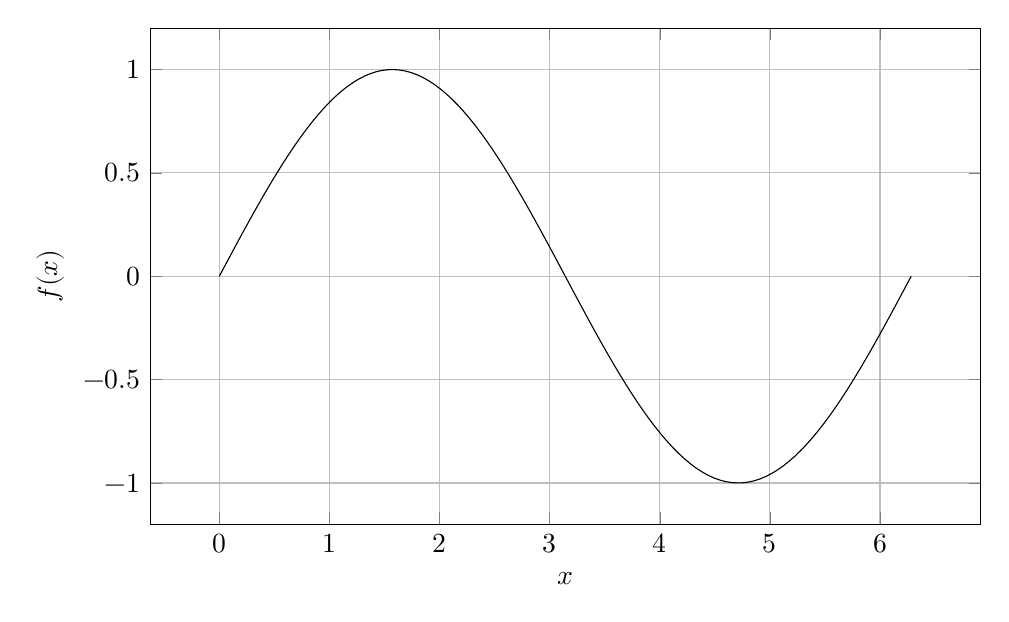
\begin{tikzpicture}
\begin{axis}[
    width=\columnwidth,
    height=0.65\columnwidth,
    xlabel={$x$},
    ylabel={$f(x)$},
    grid=major
]
\addplot[
    domain=0:6.28318,
    samples=120
]
{sin(deg(x))};
\end{axis}
\end{tikzpicture}
\caption{A simple PGFPlots sine curve.}
\end{figure}

SVG files can be included with the \texttt{svg} package:

\begin{center}
\texttt{\textbackslash includesvg[width=0.8\textbackslash columnwidth]\{device\}}
\end{center}

For example, if \texttt{device.svg} is in the same folder, use:

\begin{figure}[h]
\centering
% Requires: latexmk -lualatex -shell-escape this-file.tex
% Requires Inkscape installed.
% Uncomment when device.svg exists:
% \includesvg[width=0.8\columnwidth]{device}
\fbox{\parbox{0.75\columnwidth}{\centering SVG placeholder}}
\caption{Example SVG graphic placeholder.}
\end{figure}

\section{A Compact Reading Example}

Consider the statement
\[
\forall \vct{x}\in\R^n,
\qquad
\norm{\vct{x}}=0
\Leftrightarrow
\vct{x}=\vct{0}.
\]

This reads:

For every vector \(\vct{x}\) in \(\R^n\), the norm of \(\vct{x}\) is zero
if and only if \(\vct{x}\) is the zero vector.

Another compact statement is
\[
\forall \epsilon>0,
\quad
\exists \delta>0
\quad
\text{such that}
\quad
\abs{x-a}<\delta
\Rightarrow
\abs{f(x)-f(a)}<\epsilon.
\]

This is the symbolic structure of continuity.

\section{Notation Summary}

\begin{table*}[t]
\centering
\caption{Summary of common mathematical notation.}
\begin{tabular}{lll}
\toprule
Category & Symbol & Meaning \\
\midrule
Numbers & $\N,\Z,\Q,\R,\C$ & natural, integer, rational, real, complex numbers \\
Logic & $\forall,\exists,\exists!$ & for all, exists, exists exactly one \\
Logic & $\Rightarrow,\Leftrightarrow$ & implies, if and only if \\
Sets & $x\in A$ & \(x\) is an element of \(A\) \\
Sets & $A\subseteq B$ & \(A\) is a subset of \(B\) \\
Vectors & $\vct{x}\in\R^n$ & real vector of length \(n\) \\
Matrices & $\mat{A}\in\R^{m\times n}$ & real \(m\)-by-\(n\) matrix \\
Linear algebra & $\mat{A}\T,\mat{A}^{-1}$ & transpose, inverse \\
Linear algebra & $\tr(\mat{A}),\determinant(\mat{A})$ & trace, determinant \\
Calculus & $\dv{y}{x},\pdv{f}{x}$ & ordinary and partial derivatives \\
Vector calculus & $\grad,\divg,\curlop,\Delta$ & gradient, divergence, curl, Laplacian \\
Complex & $\ii^2=-1$ & imaginary unit \\
Fourier & $\FT,\IFT$ & Fourier transform and inverse transform \\
Probability & $\E,\Var,\Cov$ & expectation, variance, covariance \\
Statistics & $\Normal(\mu,\sigma^2)$ & Gaussian distribution \\
Spaces & $L^2,H^1,C^\infty$ & function spaces \\
Rotations & $SO(3)$ & 3D rotation matrix group \\
Quaternions & $q_1\otimes q_2$ & quaternion product \\
Numerics & $\bigO(h^p)$ & asymptotic error order \\
\bottomrule
\end{tabular}
\end{table*}

\section{Conclusion}

Mathematical notation is a compact way to express relationships between
objects. The most important habit is to identify the type of each symbol:
scalar, vector, matrix, tensor, function, operator, set, space, random
variable, or process. Once the type is clear, most expressions become much
easier to read.

\end{document}
